\documentclass[12pt,a4paper]{jarticle}
\usepackage[top=35truemm, bottom=35truemm, left=30truemm, right=30truemm]{geometry}
\usepackage[dvipdfmx]{graphicx}
\usepackage[version=3]{mhchem}
\setcounter{tocdepth}{\maxdimen} %subsubsectionまで目次を表示する
\bibliographystyle{junsrt} %参照のスタイル
\makeatletter
\renewcommand{\theequation}{% 式番号の付け方
\thesection.\arabic{equation}}
\@addtoreset{equation}{section}

\renewcommand{\thefigure}{% 図番号の付け方
\thesection.\arabic{figure}}
\@addtoreset{figure}{section}

\renewcommand{\thetable}{% 表番号の付け方
\thesection.\arabic{table}}
\@addtoreset{table}{section}
\makeatother


\begin{document}
\begin{titlepage}
\title{\vspace{60mm} \LARGE 修士論文\vspace{10mm}\\J-PARC E07実験におけるbeam照射及び\\原子核乾板中の$\Xi$-粒子飛跡自動追跡}
\author{\Large 岐阜大学大学院 教育学研究科 \\ \vspace{5mm}
\Large 総合教科教育専攻 仲澤研究室 \\ \vspace{5mm}
\LARGE 後藤 良輔}
\date{最終更新 \today}
\maketitle
\thispagestyle{empty} %ページ番号を消す
\end{titlepage}

\thispagestyle{empty} %ページ番号を消す
\tableofcontents
\thispagestyle{empty} %ページ番号を消す
\newpage
\section{序論}
\subsection{はじめに}
私たちを含め、身の回りの物質は原子からできている。
その原子核は原子核と電子から構成されており、原子核は陽子と中性子で成り立つ。
さらに、陽子や中性子はクォークで構成されている。
\par
クォークは、up(u)、down(d)、strange(s)、charm(c)、top(t)、bottom(b)の6種類がある。(以降は()内の文字で省略する。)
uとd以外のクォークを含む粒子は非常に寿命が短いため地球上に存在していない。
私たちはsクォークを含む粒子の相互作用について研究を進めている。
\par
sクォークを含む粒子の相互作用を調べる理由として中性子星がある。
中性子星は直径が約10kmでその質量が太陽の約1~2倍と非常に高密度な星である。
そのため、中性子星の平均密度は原子核の平均密度の約2.5倍となる。
\par
図\ref{fig:den_barion}は密度に対する粒子の存在量を示している。
通常の原子核の密度領域では中性子(n)、陽子(p)が存在している。
しかし、図中の青の領域で示した中性子星の密度領域では、n、pに加えてsクォークを含む$\Lambda$、$\Xi$$^-$が存在することが図から分かる。
これは、中性子星内部のpの量が増大すると、nの化学ポテンシャルが$\Lambda$の化学ポテンシャルを上回るようになり、
nが$\Lambda$に変位する方がエネルギー的に安定するため起こる。
そのため、中性子星の内部構造を探るためにはsクォークを含む$\Lambda$、$\Xi$$^-$から粒子間の相互作用を求めることが必要である。
\par
一般に粒子の相互作用を調べるためには粒子同士の衝突散乱実験を行うが、
私たちの研究で使用する$\Lambda$粒子はudsの3つのクォークからなり、その寿命は10$^-$$^1$$^0$秒であるため、
衝突実験によって相互作用を知ることは不可能である。
そのため、$\Lambda$粒子の相互作用を求めるには原子核の中に$\Lambda$粒子を持つものを生成し、核の崩壊過程から相互作用を求めるという手法しかない。
我々はハイパー核の生成、崩壊過程に関する研究を進めている。
\begin{figure}[htbp]
  \centering
   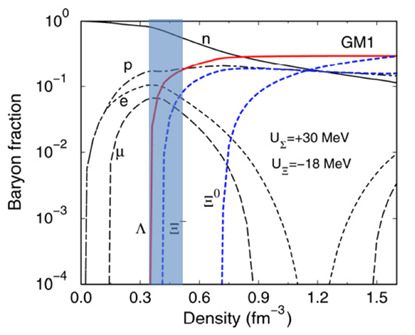
\includegraphics[width=70mm]{den_barion.png}
  \caption{密度に対する粒子の存在量\label{fig:den_barion}}
\end{figure}
\subsection{Double-$\Lambda$Hyper核}
通常の核に$\Lambda$粒子を2つ持たせたものがDouble-$\Lambda$Hyper核である。
Double-$\Lambda$Hyper核を生成するため、K$^+$,K$^-$反応により$\Xi$$^-$粒子を生成する。
K$^+$,K$^-$反応は式(\ref{eq:K+-})の反応である。
そして、生成された$\Xi$$^-$粒子を原子核に吸収させることで式(\ref{eq:Xi_eq})の反応を起こし$\Lambda$粒子を生成する。
\begin{equation}
	\ce{K- + p -> $\Xi$- + K+}
\label{eq:K+-}
\end{equation}
\begin{equation}
	\ce{$\Xi$- + p -> $\Lambda$ + $\Lambda$ + 28.6Mev}
\label{eq:Xi_eq}
\end{equation}
\par
E07実験では、K$^-$粒子を生成しDiamond Targetに照射することで$\Xi$$^-$粒子を生成する。
そして、生成された$\Xi$$^-$粒子を原子核乾板中で静止させる。
$\Xi$$^-$粒子は電離損失により$\Xi$$^-$粒子の持つエネルギーが減少していく。
エネルギーが減少した後に乾板中の原子核に吸収されることで、核内の陽子と反応を起こす。
これらの反応により生成された2つの$\Lambda$粒子が原子核の中にとどまると、Single-$\Lambda$Hyper核やDouble-$\Lambda$Hyper核が生成される。
\par
E07実験では上述したとおり原子核乾板の外で$\Xi$$^-$粒子を生成し、乾板中で$\Xi$$^-$粒子を反応させる。
しかし、それ以外にもK$^-$粒子が原子核乾板の中の原子核と反応しDouble-$\Lambda$Hyper核ができる場合もある。
\par
\begin{figure}[htbp]
  \centering
     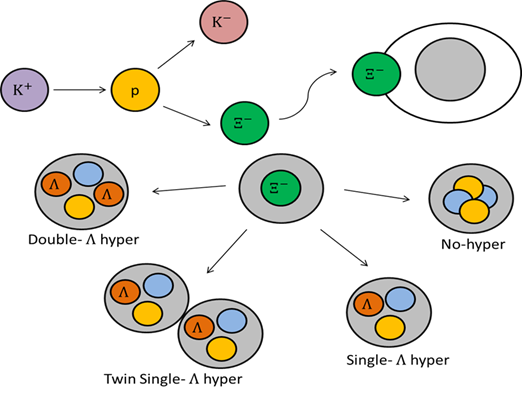
\includegraphics[width=120mm]{makehyper.png}
  \caption{Hyper核生成過程\label{fig:makehyper}}
\end{figure}
\newpage
\subsection{原子核乾板}
原子核乾板とは非常に高感度な写真フィルムの一種で、荷電粒子の通過した跡を記録する検出器である。
私たちが実験で使用する$\Lambda$粒子の寿命は非常に短いため、Hyper核の生成・崩壊事象をすべて記録できる原子核乾板を使う必要がある。
\par
原子核乾板はBaseと呼ばれるポリスチレンフィルムで作成された支持体にEmulsionを塗布して作成している。
Emulsionは通常の写真乳剤よりもハロゲン化銀の含有量が高く,最小電離損失に対して感度を持っているものである。
E07実験で使用する原子核乾板1400枚(薄型:200、厚形:1200)はすべて岐阜大学で製造された。
\par
E07実験で使用する乾板は40 µmのBaseに450 µmの乳剤を塗布する厚型乾板と、180 µmのBaseに100 µmの乳剤を塗布する薄型乾板の二種類である。
\par
薄型乾板はSSDとemulsionとの接続に使用される。
薄型乾板はbaseが厚く、乳剤が薄く塗布されているため現像の前後で乾板の変形が小さい。
そのため、記録された飛跡の角度や位置を明確に求められる。
\par
厚形乾板は照射された$\Xi$粒子を乾板中で静止させ、娘粒子の飛跡を記録するために用いられる。
そのため、荷電粒子飛跡が記録されないbaseを薄くし、乳剤の塗布量を多くすることでハイパー核事象の全飛跡を乾板中で記録する。
\par
\begin{figure}[htbp]
  \centering
     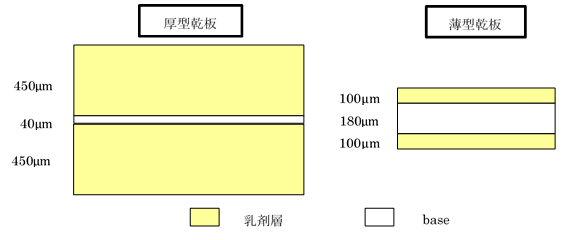
\includegraphics[width=140mm]{emulsionorder.png}
  \caption{使用する原子核乾板の規格\label{fig:emulsionorder}}
\end{figure}
\par
\newpage
原子核乾板の利点としては大きく分けて2点ある。
\par
一点目は、現像処理を行うことで半永久的に顕微鏡による観測を可能にすることである。
原子核乾板中を荷電粒子が通ることで、原子核乾板の主成分であるAgBrが電離され銀原子が生成される。(図\ref{fig:process_recored_track}(a))
現像処理により、銀が成長し1µm程度の粒となり(grain)、荷電粒子の飛跡がgrainの連なり(track)として現れ、その状態を保持する。(図\ref{fig:process_recored_track}(b))
そのため、原子核乾板を破損しない限り一度記録したHyper核の生成・崩壊事象やHyper核以外の荷電粒子秘跡を何度でも同じ状態で観測することができる。
\par
二点目は、サブミクロン精度での空間分解能を持つことである。
生成される銀粒子の大きさが$\mu$mオーダーのため、その大きさでの位置分解能が出る。
また、乾板に記録された飛跡の長さ、太さは通過した荷電粒子のエネルギーや電荷に依存する。
そのため、私たちは記録されたHyper核事象の飛跡の長さと角度からエネルギーを計算することで$\Lambda$-$\Lambda$間に働く相互作用を算出することができる。
\begin{figure}[htbp]
  \centering
      \begin{tabular}{c}
        % 1枚目の画像
        \begin{minipage}{0.5\hsize}
          \centering
            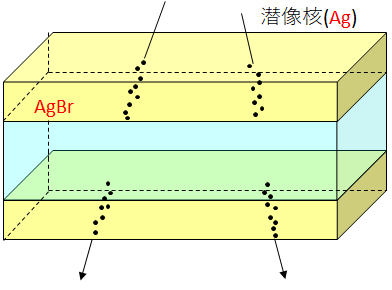
\includegraphics[clip, width=60mm]{process_bdev.png}
            \hspace{1.6cm} (a)現像前
        \end{minipage}
        
        % 2枚目の画像
        \begin{minipage}{0.5\hsize}
          \centering
            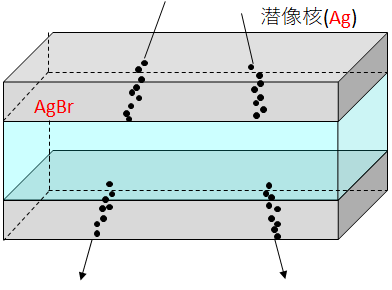
\includegraphics[clip, width=60mm]{process_adev.png}
            \hspace{1.6cm} (b)現像後
        \end{minipage}
    
      \end{tabular}
      \caption{原子核乾板中に飛跡が記録される過程の模式図\label{fig:process_recored_track}}
\end{figure}
\begin{figure}[htbp]
 \centering
      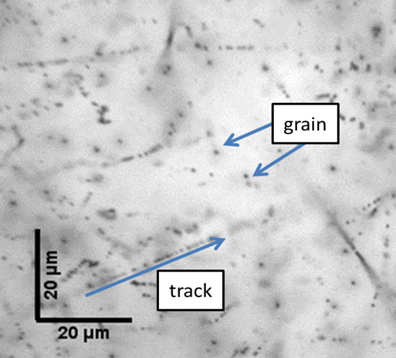
\includegraphics[width=70mm]{grainfog.png}
 \caption{原子核乾板中に記録されるtrackとgrain\label{fig:grain_track}}
\end{figure}
\subsection{光学顕微鏡}
光学顕微鏡を用いて、現像後の原子核乾板に記録されているtrackを追跡、観察する。
使用する顕微鏡は、モーターによって水平方向(x、y方向)に約1µmの精度で位置制御し、エンコーダーによって鉛直方向(z方向)に約0.1 µmの精度で稼働できる。
この顕微鏡により、原子核乾板表面の推測される位置で目的のtrackを探し、$\Xi$$^-$粒子候補を見つけ、trackを原子核乾板上面から下面まで追跡していく。
\par
PCを接続することで、この光学顕微鏡を制御している。
CCDカメラを顕微鏡に設置することで、顕微鏡で観察したものを画像として取得する。
取得した画像をPCの画面上に表示することや、顕微鏡の稼働に活用している。
$\Xi$$^-$粒子自動追跡には、50倍の対物レンズを使用している。
ここにx,y,zの精度を書けたらいいかな。
\begin{figure}[htbp]
  \centering
     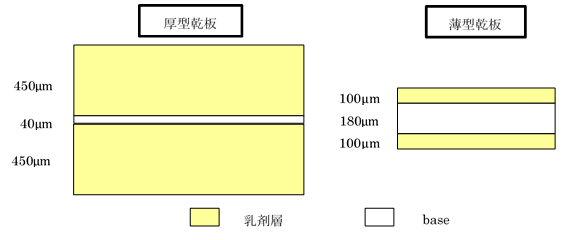
\includegraphics[width=140mm]{emulsionorder.png}
  \caption{光学顕微鏡\label{fig:microscope}}
\end{figure}
\newpage
\subsection{KEK-PS E373実験}
E373実験はE176実験に続くDouble-$\Lambda$Hyper核検出実験である。
\cite{Nagara}
\cite{Nagara2}
E176実験の約10倍のDouble-$\Lambda$Hyper核の検出を目標にし、エマルジョンとカウンターを組み合わせたハイブリッド-エマルジョン法を取り入れて実施された。
約1000の$\Xi$$^-$粒子吸収事象が見積もられ、光学顕微鏡を用いた半自動飛跡追跡により全モジュールの解析が終了している。
解析の結果、ハイブリッド-エマルジョン法により約600例の$\Xi$$^-$粒子吸収事象を検出し、7例のDouble-$\Lambda$Hyper核を検出した。
その中の1例でのみ崩壊モードを一意に決定することができ、この1例をNAGARA Eventと名付けた。
\begin{figure}[htbp]
  \centering
      \begin{tabular}{c}
        % 1枚目の画像
        \begin{minipage}{0.5\hsize}
          \centering
            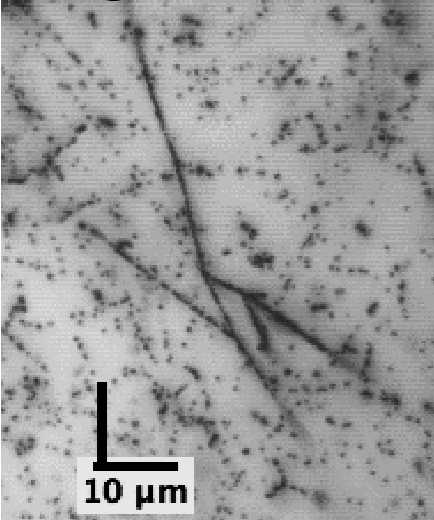
\includegraphics[clip, width=40mm]{Nagara.png}
            \hspace{1.6cm} 
            \caption{Nagara event\label{fig:Nagara}}
        \end{minipage}
        
        % 2枚目の画像
        \begin{minipage}{0.5\hsize}
          \centering
            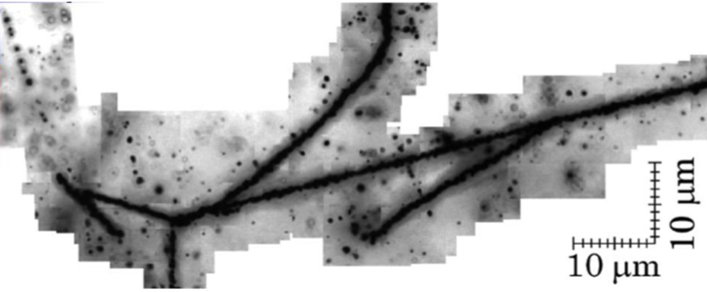
\includegraphics[clip, width=70mm]{Kiso.png}
            \hspace{1.6cm} 
            \caption{Kiso event\label{fig:Kiso}}
        \end{minipage}
    
      \end{tabular}
\end{figure}
\subsection{J-PARC E07実験}
J-PARC E07実験はハイブリッド-エマルジョン法によりKEK-PS E373実験の10倍の統計量を目指す実験である。
表\ref{tab:compare_E07_E373}はJ-PARC E07実験とKEK-PS E373実験の比較をしたものである。
表にあるように、beamのK$^-$/$\pi$$^-$を約3.5倍、原子核乳剤の量を約3倍にすることで10倍の$\Xi$$^-$粒子静止事象を実現する。
\par
E07実験ではカウンターとしてSSDを採用している。
SSDは電荷をもった粒子が通過した際に、通過した粒子が原子核乾板スタックのどの位置にどのような角度で照射されているかの情報を記録する検出器である。
SSDは4層構造になっているため、同タイミングで4層に渡って検出された座標情報を使い、通過した荷電粒子の角度を推定することができる。
原子核乾板スタックを2つのSSDで挟むことで、Diamond Targetで生成された$\Xi$$^-$粒子だけでなく、原子核乾板内で反応した$\Xi$$^-$粒子の情報も記録できる。
SSDの情報を使い、emulsionに記録された飛跡の中で$\Xi$$^-$粒子である確率の高い飛跡のみを追跡することでいち早くDouble-$\Lambda$Hyper核を検出する。
SSDの精度と前回の検出器の精度の違いを示す。
\begin{table}[htbp]
\centering
\caption{J-PARC E07実験とKEK-PS E373実験の比較\label{tab:compare_E07_E373}}
\begin{tabular}{c|c|c}
   &KEK-PS E373実験&J-PARC E07実験\\
\hline
\hline
$\Xi$$^-$粒子静止事象 & ~10$^3$    & ~10$^4$  \\
K$^-$/$\pi$$^-$ & 1/4  & 6/1 \\
原子核乳剤量 & 0.8t & 2.1t  \\
\hline
\end{tabular}
\end{table}
\begin{table}[htbp]
\centering
\caption{原子核乾板中に記録されるtrackとgrainの様子\label{tab:grain_track}}
\begin{center}
    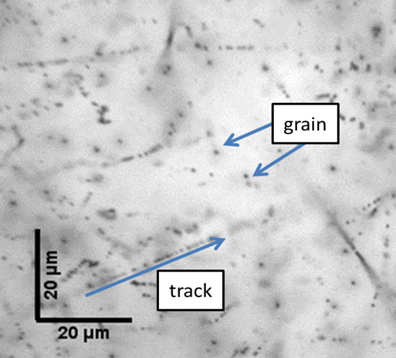
\includegraphics[width=70mm]{grainfog.png}
\end{center}
\end{table}


\newpage
\section{J-PARC E07実験2ndRun}
J-PARC E07実験は1stRunを2016年6月18日〜30日に、2ndRunを2017年5月~7月に実施した。
1stRunでは18stacks、2ndRunでは100stacksのbeam照射に成功した。
beam照射を行うにあたり使用する原子核乾板のバックグラウンド削減法の実施、原子核乾板の真空パック法の確立、現像等を実施した。
\par
本章ではJ-PARC E07実験beam照射、現像においての実施内容及びその手法について述べる。
強制現像退行処理と原子核乾板の現像に関する詳細な情報及び処理の評価については大橋修士論文に記載する。
\subsection{Refresh処理の実施}
\subsubsection{実施背景}
J-PARC E07実験で使用する原子核乾板約1400枚はすべて岐阜大学ダブルハイパー核実験棟にて制作した。
制作は2013年12月~2014年3月の期間で完了している。
当初の予定では乾板製造後すぐにbeam照射を実施する予定であったが、J-PARCでの放射能漏れ事故により実験は延期になった。
\par
製造した原子核乾板は現像されるまで空気中の宇宙線やコンプトン電子を記録していく。
図\ref{fig:compton_and_cosmicray_in_emulsion}は原子核乾板中に記録されたコンプトン電子と宇宙線を示している。
これらのgrainや飛跡がバックグラウンドとして増加すると、beam照射後の解析に支障を来す恐れがある。
そこで、宇宙線の影響が少ない神岡鉱山内に鉛ブロックで箱を作り、製造した原子核乾板を保管した。(図\ref{fig:emulsion_in_Kamioka})
\par
図\ref{fig:stragecompton}は製造からの時間経過による原子核乾板記録された宇宙線、コンプトン電子の増加傾向を示している。
赤色が岐阜大学の冷蔵庫内で保管した場合、青色が神岡鉱山鉛箱内で保管した場合である。
二つの線の傾きを比較すると、神岡鉱山内で保管したことで非常に多くのバックグラウンドを削減することができたということが分かる。
\par
しかし、製造からbeam照射まで2年の期間が経過したため、神岡鉱山内で保管していたとしても解析に支障を及ぼすレベルまでバックグラウンドが蓄積してしまった。
図\ref{fig:beam_efficiency_to_compton}はコンプトンの蓄積量に対するbeam検出効率を示したものである。
制作から約2年間経過した原子核乾板には期間中神岡鉱山内で保管した場合、バックグラウンドが●●となる。
図からバックグラウンドが●●となると、beam検出効率が著しく低下することが分かる。
そのため、蓄積されたバックグラウンドの消去のために原子核乾板に対して強制潜像退行処理(Refresh処理)を実施した。
\par
\begin{figure}[htbp]
  \centering
      \begin{tabular}{c}
        % 1枚目の画像
        \begin{minipage}{0.5\hsize}
          \centering
            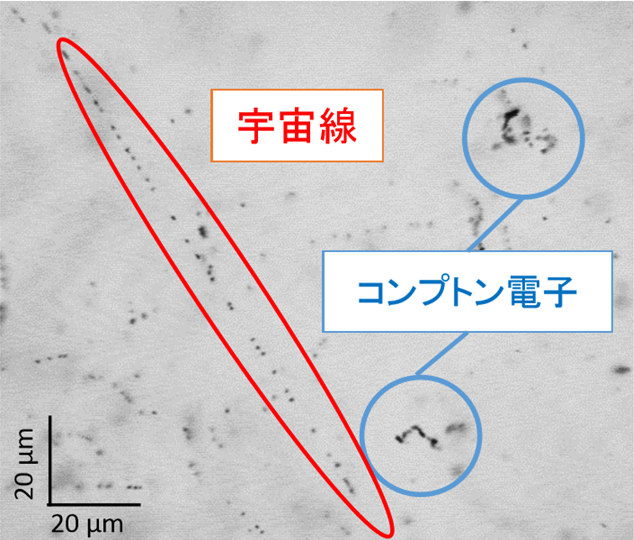
\includegraphics[clip, width=70mm]{compton_cosmiclay.png}
            \hspace{1.6cm} 
            \caption{乾板に記録されたコンプトン電子と宇宙線の飛跡\label{fig:compton_and_cosmicray_in_emulsion}}
        \end{minipage}
        
        % 2枚目の画像
        \begin{minipage}{0.5\hsize}
          \centering
            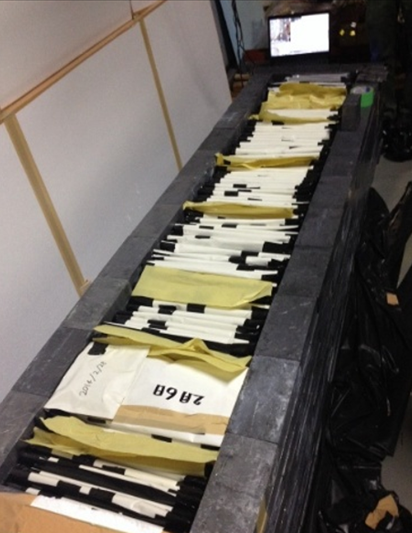
\includegraphics[clip, width=50mm]{emulsion_in_Kamioka.png}
            \hspace{1.6cm} 
            \caption{神岡鉱山内の鉛ブロック中に原子核乾板の保管状況\label{fig:emulsion_in_Kamioka}}
        \end{minipage}
    
      \end{tabular}
\end{figure}
\begin{figure}[htbp]
  \centering
     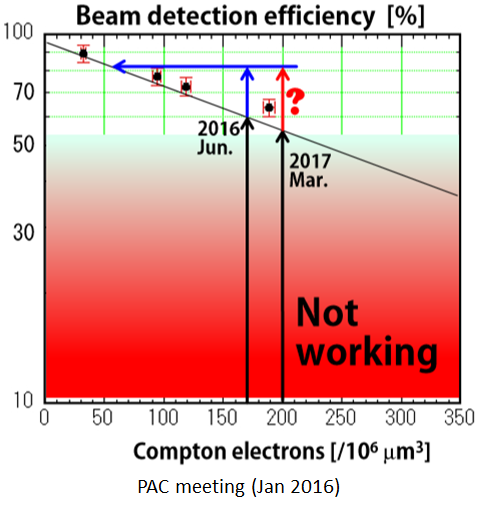
\includegraphics[width=70mm]{beam_efficiency_to_compton.png}
  \caption{保管地点によるコンプトンの蓄積量\label{fig:stragecompton}}
\end{figure}
\begin{figure}[htbp]
  \centering
     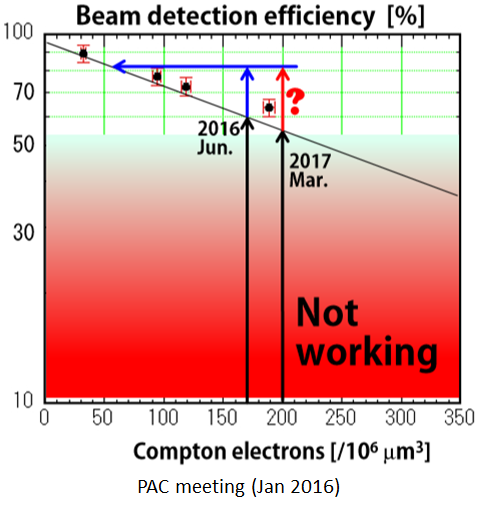
\includegraphics[width=70mm]{beam_efficiency_to_compton.png}
  \caption{コンプトンの蓄積量に対するbeamの検出効率\label{fig:beam_efficiency_to_compton}}
\end{figure}
\newpage
\subsubsection{原理}
写真フィルムには撮影してから現像するまでに時間を経ると、映像が消えていく性質(潜像退行性)がある。[式(\ref{eq:gennzou})]
また、潜像退行性は高温高湿度の環境で著しく進むことが明らかになっている。
\begin{equation}
    \ce{Ag4 + O2 + 2H2O -> 4Ag+ + 4OH-}
\label{eq:gennzou}
\end{equation}
\par
原子核乾板は塗布されてから現像されるまでの間に、自然放射線や宇宙線の影響を受け潜像が蓄積される。
そこで、蓄積された潜像を消去するための手法として強制潜像退行処理(Refresh処理)と呼ばれる方法が開発されている。
\cite{takusann}
Refresh処理は原子核乾板の持つ現像退行性を利用する。
図\ref{fig:intr_refresh}はRefresh処理の模式図である。
原子核乾板には荷電粒子が通過した跡に対して潜像核が形成されている。(図\ref{fig:intr_refresh}(a))
原子核乾板中に記録された潜像核に対して式\ref{eq:gennzou}の反応を起こすことで、形成されていた潜像核がイオンになり現像されない状態になる。
(図\ref{fig:intr_refresh}(b))
この化学反応は温度が高くなるほど反応が促進されるため、原子核乾板を高温高湿度の環境下に置くことで潜像退行が促進される。
よって、Refresh処理によりbeam照射の前に記録されたBackgroundを消去できる。(図\ref{fig:intr_refresh}(c))
\begin{figure}[htbp]
  \centering
      \begin{tabular}{c}
        % 1枚目の画像
        \begin{minipage}{0.33\hsize}
          \centering
            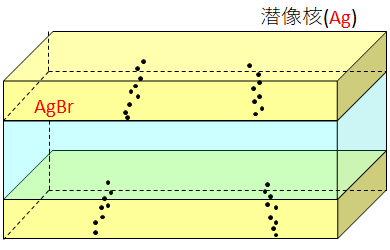
\includegraphics[clip, width=50mm]{ref_pro1.png}
            \hspace{1.6cm} (a)Refresh処理前
        \end{minipage}
        
        % 2枚目の画像
        \begin{minipage}{0.33\hsize}
          \centering
            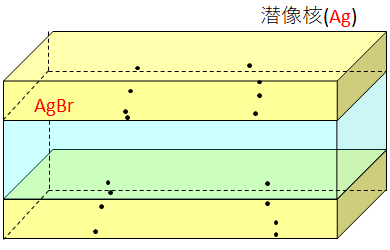
\includegraphics[clip, width=50mm]{ref_pro2.png}
            \hspace{1.6cm} (b)Refresh処理後
        \end{minipage}

        % 3枚目の画像
        \begin{minipage}{0.33\hsize}
          \centering
            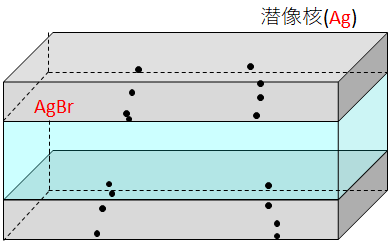
\includegraphics[clip, width=50mm]{ref_pro3.png}
            \hspace{1.6cm} (c)現像後
        \end{minipage}
    
      \end{tabular}
      \caption{Refresh処理模式図\label{fig:intr_refresh}}
\end{figure}
\subsubsection{実施環境}
E07実験で使用する原子核乾板に対してRefresh処理を実施場合は温度25度、湿度90%の環境を維持することが必要である。[大橋卒論]
そこで、温度と湿度をコントロールするチェンバーを作成した。(図\ref{fig:refresh_masi-nn})
このチェンバーは1度の処理で100枚の原子核乾板のRefresh処理を実施可能である。
1stRunではこの装置を使い4回のRefresh処理を実施し、温度湿度の制御を手動で行った。
2ndRunでは13回のRefresh処理を、温度・湿度の調整を自動制御で実施した。[村本卒論]
\begin{figure}[htbp]
  \centering
     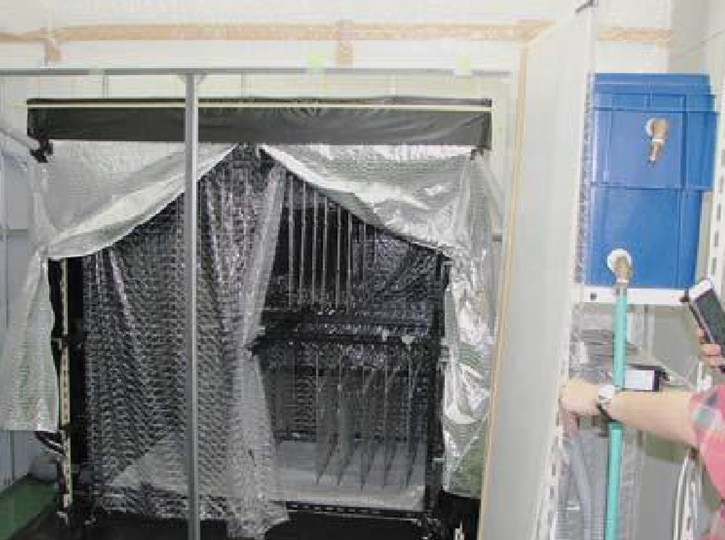
\includegraphics[width=100mm]{refresh_chember.png}
  \caption{Refreshチェンバー\label{fig:refresh_masi-nn}}
\end{figure}
\begin{figure}[htbp]
  \centering
      \begin{tabular}{c}
        % 1枚目の画像
        \begin{minipage}{0.5\hsize}
          \centering
            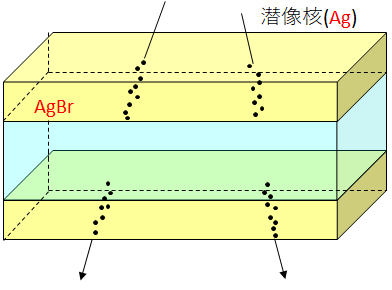
\includegraphics[clip, width=60mm]{process_bdev.png}
            \hspace{1.6cm} (a)加湿器
        \end{minipage}
        
        % 2枚目の画像
        \begin{minipage}{0.5\hsize}
          \centering
            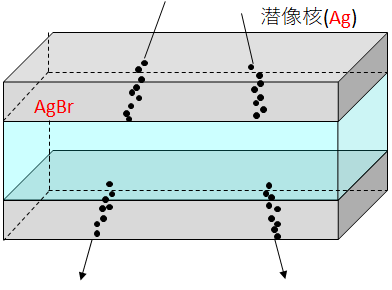
\includegraphics[clip, width=60mm]{process_adev.png}
            \hspace{1.6cm} (b)除湿器
        \end{minipage}
    
      \end{tabular}
      \caption{Refreashに使用した加湿器・除湿器\label{fig:refresh_mizumasi-nn}}
\end{figure}
\subsection{GridMark照射環境の最適化}
\subsubsection{暗室の拡張}
1stRunではbeam照射後の原子核乾板を岐阜に持ち帰り、現像の数日前に岐阜でGridマークを照射した。
beam照射からGridマーク照射までの間に乾板の変形があったせいか、Gridマークの位置ズレが一様でなかったため一視野内に飛跡を持ってくることが困難になった。
そこで、2ndRunではbeam照射後の原子核乾板に対してJ-PARC内の暗室下でGridMark照射を実施した。
そのため2017年3月にGridMark照射装置を設置するため暗室の拡張を行った。
\par
図\ref{fig:darkroom}は暗室拡張後を示したものである。
横の長さを1m拡張することで、Gridマーク照射装置を設置する場所を確保した。
\begin{figure}[htbp]
  \centering
    \begin{tabular}{c}
      % 1枚目の画像
      \begin{minipage}{1.0\hsize}
        \centering
          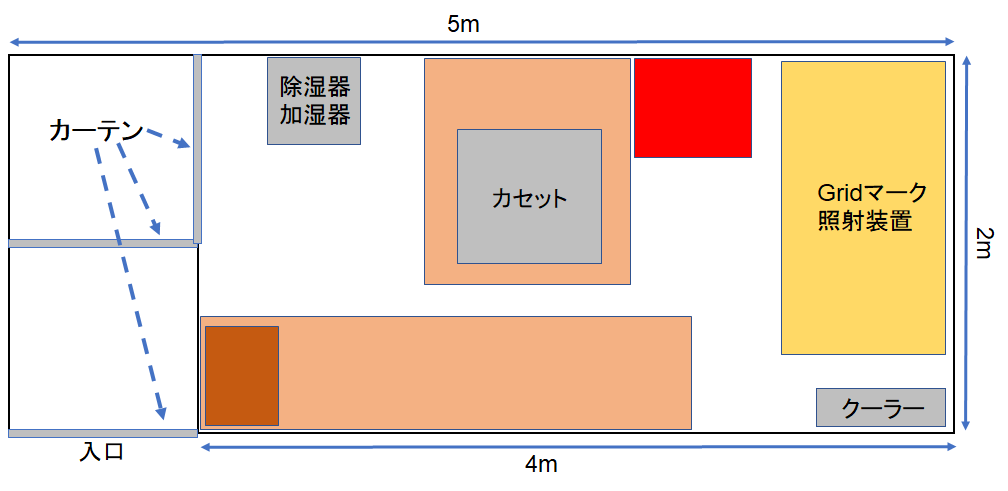
\includegraphics[clip, width=140mm]{darkroom_after.png}
          \hspace{1.6cm} (a)拡張後暗室内図
      \end{minipage}
      \\
      % 2枚目の画像
      \begin{minipage}{1.0\hsize}
        \centering
          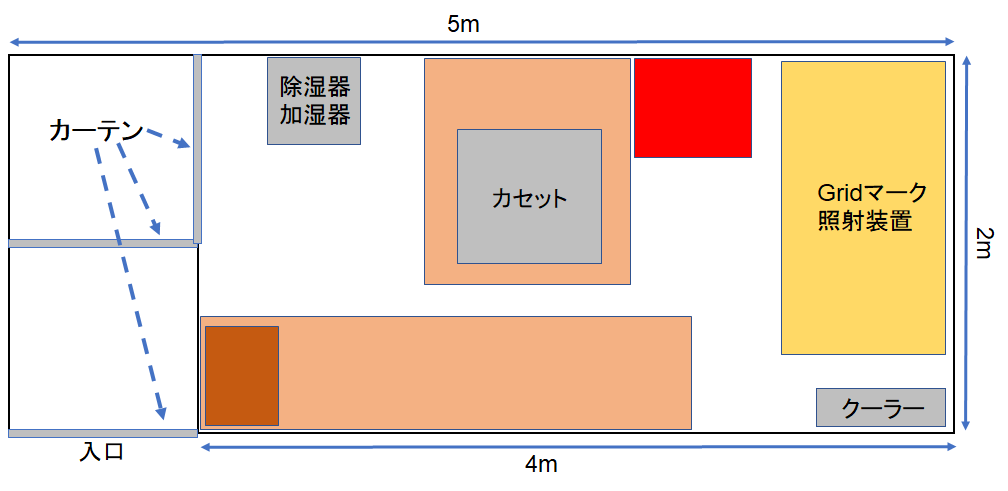
\includegraphics[clip, width=140mm]{darkroom_after.png}
          \hspace{1.6cm} (b)暗室内部
      \end{minipage}
    \end{tabular}
    \caption{暗室後\label{fig:darkroom}}
\end{figure}
\par
暗室拡張後、暗室内が原子核乾板を取り扱うのに適した環境であるかどうかを確認した。
暗室内湿度は加湿器・除湿器を設定し常時50%を超えるように設定した。(図\ref{fig:kasituki_zyosituki})
室温はクーラーにより常時20~25℃になるように設定した。
図\ref{fig:darkroom_situdo}、\ref{fig:darkroom_onndo}は暗室拡張後、湿度・温度が一定に保たれているかを確認した図である。
図\ref{fig:darkroom_situdo}、\ref{fig:darkroom_onndo}より、
暗室内は原子核乾板を取り扱うのに適した環境にできていると判断をしたうえでE07実験2ndRunを実施した。
\begin{figure}[htbp]
  \centering
      \begin{tabular}{c}
        % 1枚目の画像
        \begin{minipage}{0.5\hsize}
          \centering
            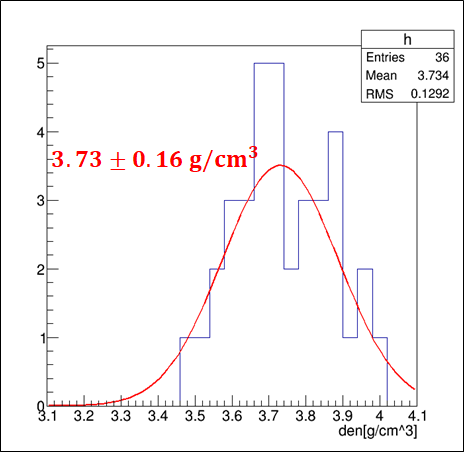
\includegraphics[clip, width=60mm]{1stRun_thin_den.png}
            \hspace{1.6cm} (a)除湿器
        \end{minipage}
        
        % 2枚目の画像
        \begin{minipage}{0.5\hsize}
          \centering
            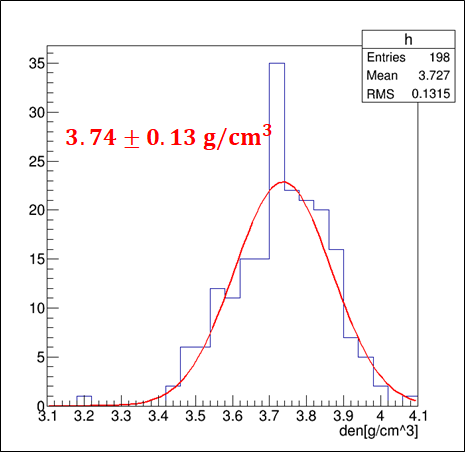
\includegraphics[clip, width=60mm]{2ndRun_thin_den.png}
            \hspace{1.6cm} (b)加湿器
        \end{minipage}
    
      \end{tabular}
      \caption{使用した除湿器、加湿器\label{fig:kasituki_zyosituki}}
\end{figure}
\begin{figure}[htbp]
  \centering
    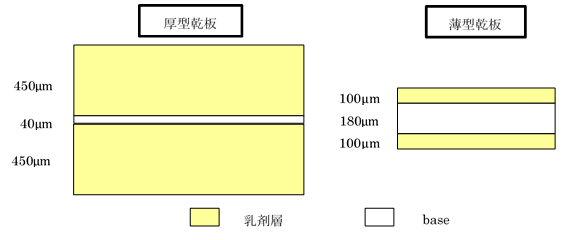
\includegraphics[width=140mm]{emulsionorder.png}
  \caption{暗室内の湿度\label{fig:darkroom_situdo}}
\end{figure}
\begin{figure}[htbp]
  \centering
    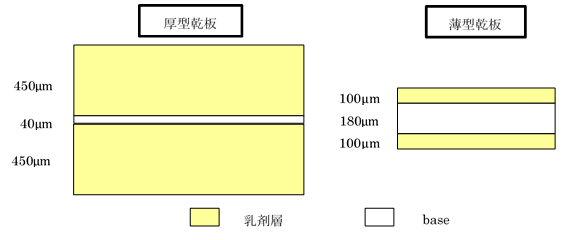
\includegraphics[width=140mm]{emulsionorder.png}
  \caption{暗室内の温度\label{fig:darkroom_onndo}}
\end{figure}
\subsubsection{GridMarkネガ}
2016年にE07実験testRunとしてbeam照射を実施した。
その際、原子核乾板に焼き付けたGridマークの中にはネガのつまりにより、Gridマークが照射されていないものが存在していた。
1stRunのGridマーク照射の際は図\ref{fig:nega_cleaner}の装置を使用してネガのつまりを除去しながら照射を行った。
しかし、1stRunの原子核乾板においてもGridマークが照射されていない箇所が存在した。
これらを受けてネガの変更を行った。
2ndRunでは2種類の素材の加工を●●に依頼し、加工と原子核乾板に対する影響の面を考慮してネガの素材を●に決定した。
E07実験2ndRunの原子核乾板には図\ref{fig:nega_2ndRun}を使いGridマークを照射した。
\begin{figure}[htbp]
  \centering
    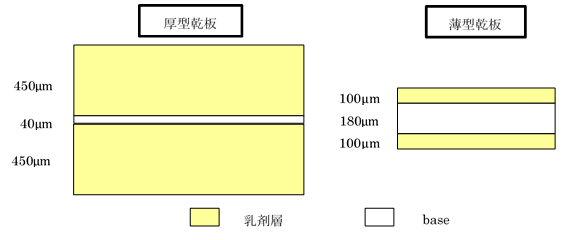
\includegraphics[width=140mm]{emulsionorder.png}
  \caption{ネガのつまり除去装置\label{fig:nega_cleaner}}
\end{figure}
\begin{figure}[htbp]
  \centering
    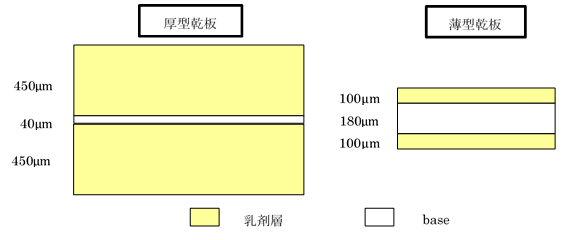
\includegraphics[width=140mm]{emulsionorder.png}
  \caption{E07実験2ndRunネガ\label{fig:nega_2ndRun}}
\end{figure}
\subsubsection{GridMark照射装置}
E071stRunではタイマーを用いて10秒間原子核乾板に露光した。
この先行研究と同様の手法(田村卒論)で1mod分照射するのに約1時間半の時間が必要になる。
E07実験2ndRunではbeam照射後すぐにGridマークを照射する。
従来の手法から変更することで照射の時間短縮及び疲労の削減のために照射装置の改造を行った。
\par
田村卒論を確認して、露光時間、最終的にどれくらい照射すれば良いのか、照射装置の構造の写真を引用して載せる。
\par
吉田氏が組んだ回路の図を載せる。
2ndRunのGridマークはこの装置を使用して焼き付けた。
田村さんの卒論からGridマークを焼き付けるのにどれくらい照射する必要があるのかを確認して引用する。
\begin{figure}[htbp]
  \centering
     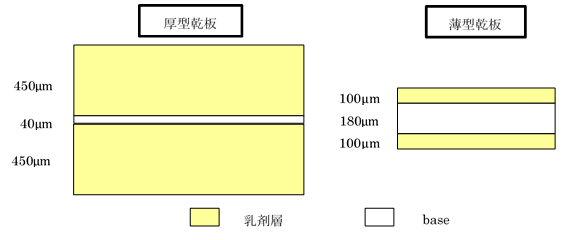
\includegraphics[width=140mm]{emulsionorder.png}
  \caption{Gridマーク照射装置\label{fig:grid_masi-nn}}
\end{figure}
\subsection{E07実験2ndRunbeam照射}
\subsubsection{作業内容}
2017年5月●日~7月●日にかけて100stacksの原子核乾板すべてにbeam照射を行った。
図\ref{fig:beam_day}から、途中beam照射が停止しながらも予定通り100modの原子核乾板にbeamを照射しきることができた。
\begin{figure}[htbp]
  \centering
     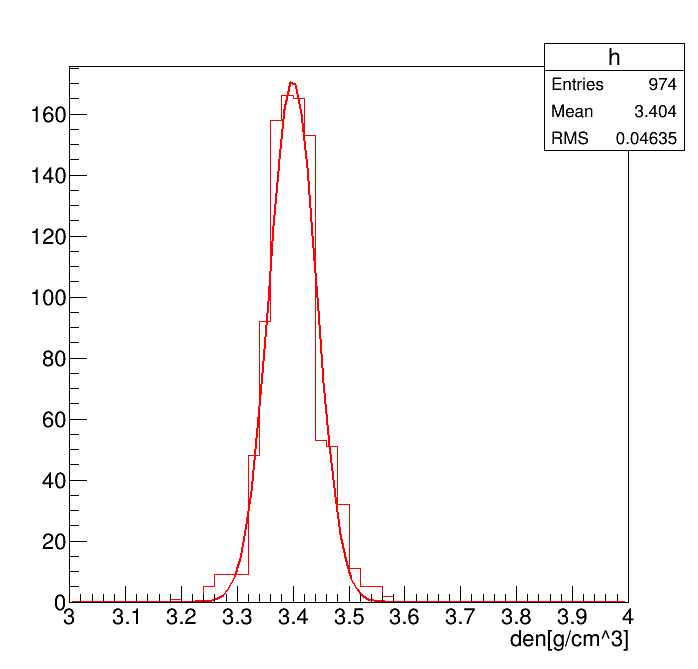
\includegraphics[width=70mm]{thick75_den.png}
  \caption{2ndRunで照射した原子核乾板の数\label{fig:beam_day}}
\end{figure}
E07実験2ndRunで岐阜大学グループは原子核乾板の取り扱いに関する部分を実施した。
暗室内で原子核乾板をEmulsionCasetteに詰める際の流れは以下の通りである。
この作業は、先行研究で確立した方法に基づいて実施した。[遠藤修論]
\begin{enumerate}
    \item beam照射8時間前に乾板を冷蔵庫から出し、常温に慣らしておく。
    \item グリスを塗った、Oリングをはめ込む。
    \item カセットの4つ角にL字のSUS板を置く。 
    \item 袋から乾板を開けて乾板の重さ・厚さを測定し、乾板の番号を記録、乾板にMOD番号を書く。
    \item 乾板をL字のSUS板に沿って原子核乾板13枚をカセットに入れる。
    \item 1.0 mm厚のSUS枠のゴム板側にシリコングリスを塗り、SUS枠をはめる。(図\ref{fig:tezyun_6})
    \item 1.0 mm厚のゴム板をはめる。(図\ref{fig:tezyun_7})
    \item 木の板を置き,その上におもりを置くことで乾板を固定した後,L字のSUS板を外す。(図\ref{fig:tezyun_8})
    \item カセットおさえを置き,ねじを軽くしめる。(図\ref{fig:tezyun_9})
    \item ねじを数回に分けてしめる。
    \item 図\ref{fig:ponpu}の水流真空ポンプで10分減圧し,1時間経過後もう一度減圧する。
\end{enumerate}
\begin{figure}[htbp]
  \centering
      \begin{tabular}{c}
        % 1枚目の画像
        \begin{minipage}{0.5\hsize}
          \centering
            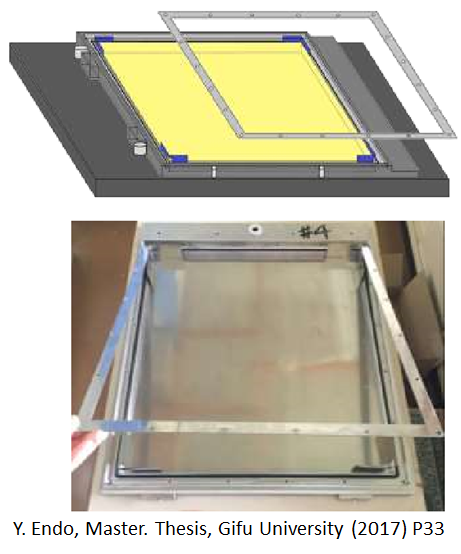
\includegraphics[clip, width=70mm]{tezyun_6.png}
            \hspace{1.6cm} 
            \caption{手順6\label{fig:tezyun_6}}
        \end{minipage}
        
        % 2枚目の画像
        \begin{minipage}{0.5\hsize}
          \centering
            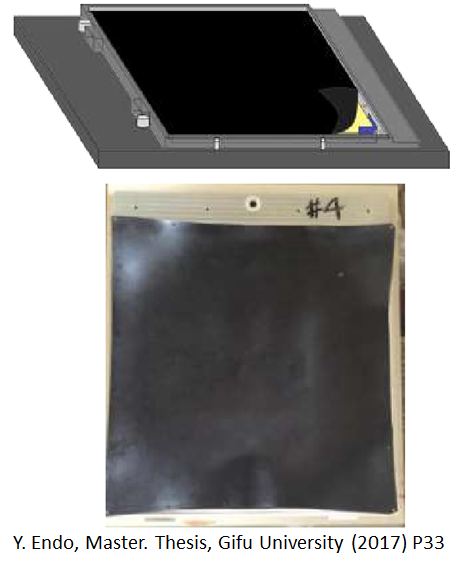
\includegraphics[clip, width=70mm]{tezyun_7.png}
            \hspace{1.6cm} 
            \caption{手順7\label{fig:tezyun_7}}
        \end{minipage}
    
      \end{tabular}
\end{figure}
\begin{figure}[htbp]
  \centering
      \begin{tabular}{c}
        % 1枚目の画像
        \begin{minipage}{0.5\hsize}
          \centering
            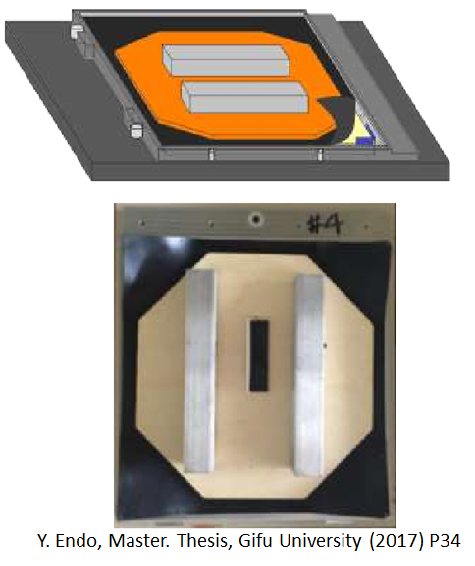
\includegraphics[clip, width=70mm]{tezyun_8.png}
            \hspace{1.6cm} 
            \caption{手順8\label{fig:tezyun_8}}
        \end{minipage}
        
        % 2枚目の画像
        \begin{minipage}{0.5\hsize}
          \centering
            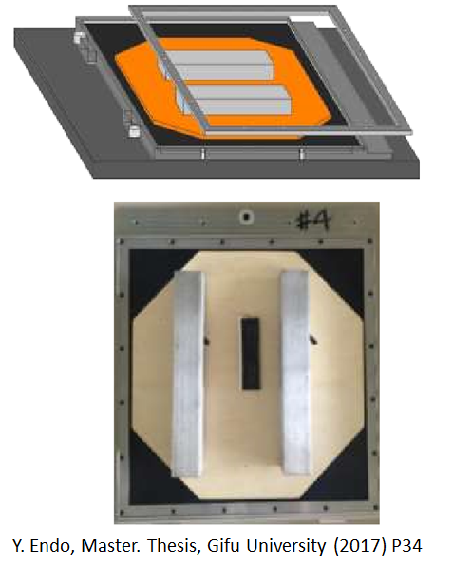
\includegraphics[clip, width=70mm]{tezyun_9.png}
            \hspace{1.6cm} 
            \caption{手順9\label{fig:tezyun_9}}
        \end{minipage}
    
      \end{tabular}
\end{figure}
\begin{figure}[htbp]
  \centering
    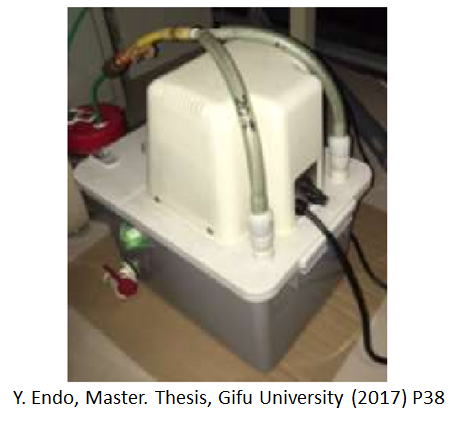
\includegraphics[width=70mm]{ponpu.png}
  \caption{水流ポンプ\label{fig:ponpu}}
\end{figure}
\newpage
\subsubsection{EmulsionCasetteでの真空度}
図\ref{fig:e07setup}はE07実験のセットアップを示したものである。
私たちは図●の暗室内にて1mod分の原子核乾板13枚(厚型:11枚、薄型2枚)を図\ref{fig:fig:casette}のEmulsionCasetteに詰めて図\ref{fig:e07setup}に示したbeamラインにセットした。
図\ref{fig:e07setup}を見れば分かるとおり、EmulsionCasetteとSSDの間には5 mmしか距離がない。
そのため、EmulsionCasetteに原子核乾板を入れ、bema照射中に適切な真空度を保つことが必要であった。
\begin{figure}[htbp]
  \centering
      \begin{tabular}{c}
        % 1枚目の画像
        \begin{minipage}{0.5\hsize}
          \centering
            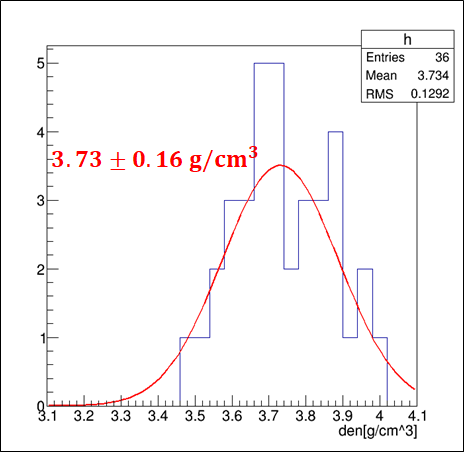
\includegraphics[clip, width=60mm]{1stRun_thin_den.png}
            \hspace{1.6cm} 
            \caption{E07セットアップ\label{fig:e07setup}}
        \end{minipage}
        
        % 2枚目の画像
        \begin{minipage}{0.5\hsize}
          \centering
            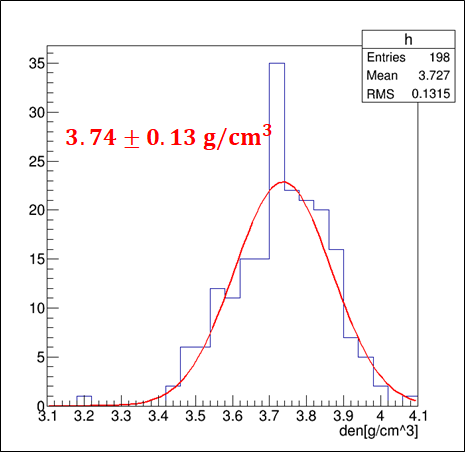
\includegraphics[clip, width=60mm]{2ndRun_thin_den.png}
            \hspace{1.6cm} 
            \caption{カセット\label{fig:casette}}
        \end{minipage}
    
      \end{tabular}
\end{figure}
\par
私たちはbeamタイム中に4台のカセットを使用し、常にストックを持ち続けながらカセットを供給することができ、
beamタイムのロスを最小限にして実験を実施できた。
beam照射直前までパッキングしたカセットの内圧をモニターし続け、Mod$\#$19~Mod$\#$118の全真空度に問題が無いことを確認したうえで、
beamラインにカセットを提供した。
Mod$\#$19~Mod$\#$118のカセットの内圧の結果を付録に記載する。
例としてMod$\#$117のカセット内圧の変化を図\ref{fig:casette_bakyu-mu}に示す。
真空度の基準は『減圧後,内圧の変化が 10 時間経過しても 0.02 MPa 以下』と先行研究で定められた。[遠藤修論]
E07実験2ndRunにおいても定められた真空度の基準をクリアしたEmulsionCasetteをbeamラインに提供した。
\begin{figure}[htbp]
  \centering
     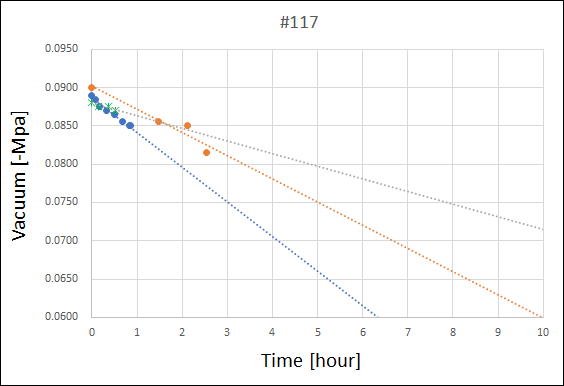
\includegraphics[width=140mm]{vacuum117.png}
  \caption{カセット内圧変化\label{fig:casette_bakyu-mu}}
\end{figure}
\subsubsection{EmulsionCasetteの固定法確立}
1stRunのbeam照射ではカセットのSUS箔が18回のカセットでの真空パックにより●回はがれた。
2ndRunのbeam照射では100回の真空引きを行う必要があるため、この頻度でSUS箔が剥がれた場合対応しきれない。
そこで、カセットのSUS箔にかかる負荷軽減のための冶具が開発された。(図\ref{fig:casette_fix})
この治具を使用して、2ndRunの照射を行った。
これにより、2ndRunでは100回の真空引きに対して1度しかSUS箔が剥がれなかった。
\begin{figure}[htbp]
  \centering
      \begin{tabular}{c}
        % 1枚目の画像
        \begin{minipage}{0.5\hsize}
          \centering
            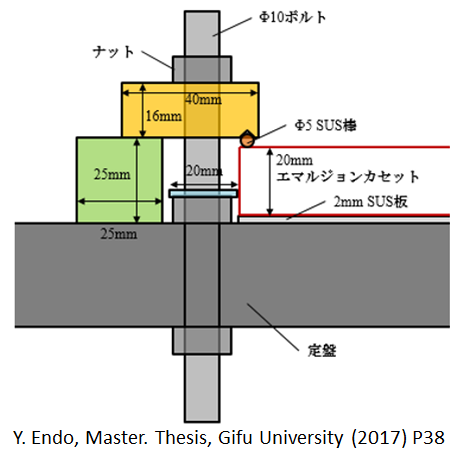
\includegraphics[clip, width=60mm]{casette_fix_moderu.png}
            \hspace{1.6cm} (a)設計図
        \end{minipage}
        
        % 2枚目の画像
        \begin{minipage}{0.5\hsize}
          \centering
            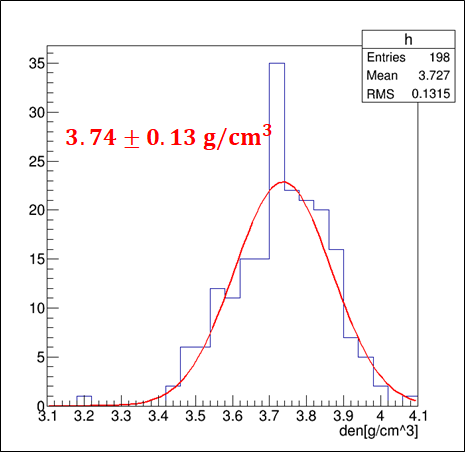
\includegraphics[clip, width=60mm]{2ndRun_thin_den.png}
            \hspace{1.6cm} (b)実物
        \end{minipage}
    
      \end{tabular}
      \caption{使用したカセット固定冶具\label{fig:casette_fix}}
\end{figure}
\newpage
\subsubsection{照射した乾板の密度}
2ndRunでは1stRunと同様にemulsionCasetteに乾板を入れる前に乾板の厚さと重さの測定、
beam照射後に乾板の重さを測定することでbeam照射により乾板の重さに大きな変動がないかを確認した。
照射の前後で重さが1.0g以上異なっていた場合は、再度厚さ重さの測定をして記録した。
乾板の重さは電子天秤を用いて、乾板の厚さはシックネスゲージを用いて乾板の4カ所を測定した。
\begin{figure}[htbp]
  \centering
      \begin{tabular}{c}
        % 1枚目の画像
        \begin{minipage}{0.5\hsize}
          \centering
            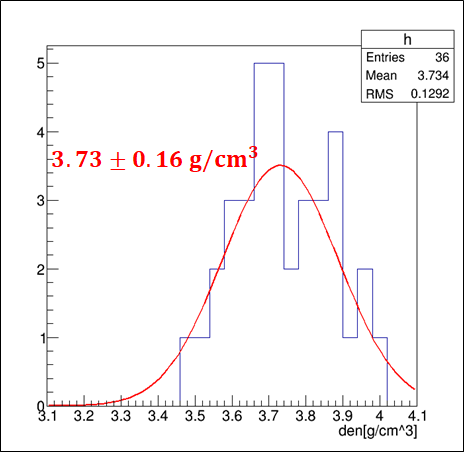
\includegraphics[clip, width=60mm]{1stRun_thin_den.png}
            \hspace{1.6cm} (a)電子天秤
        \end{minipage}
        
        % 2枚目の画像
        \begin{minipage}{0.5\hsize}
          \centering
            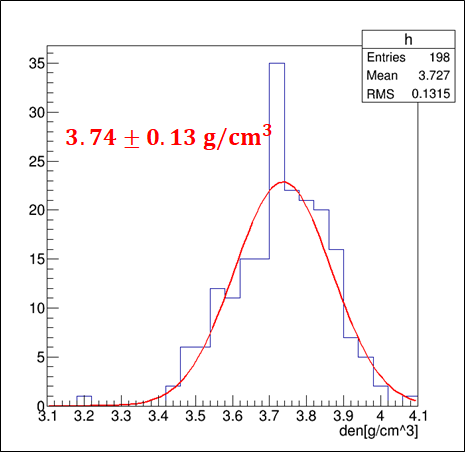
\includegraphics[clip, width=60mm]{2ndRun_thin_den.png}
            \hspace{1.6cm} (b)シックネスゲージ
        \end{minipage}
    
      \end{tabular}
      \caption{使用した電子天秤とシックネスゲージ\label{fig:tennbinn_thicknessgage}}
\end{figure}
\par
1stRun乾板の密度はRefresh未処理の乾板、2ndRunはRefresh処理実施乾板での密度で図\ref{fig:hisuto}の様にヒストグラムを作成し、
ガウスフィッティングにより密度とその誤差を求めた。
フィッティングにより算出した1stRun乾板の密度の測定結果と2ndRun乾板の密度をまとめたものが表\ref{tab:compare_E07_12}である。
比較すると、1stRunと2ndRunで使用した原子核乾板に大きな違いは無いことが分かる。
また、図\ref{fig:kasozai}はE07実験で使用する原子核乾板を作成する際に使用した可塑剤の添加量に対する原子核乾板厚型の密度を示したものである。
この図と表の数値を比較すると、可塑剤の添加量に対応した密度になっていることが分かる。
このことから、Refresh処理の有無で原子核乾板の密度が変化せず、1stRunと2ndRunで使用した原子核乾板の密度に違いは無い。
\par
薄型乾板でも同様に密度の比較をした。
表\ref{tab:compare_E07_12}を見ると、1stRunの薄型乾板は厚形乾板より密度が大きく算出されていたが、2ndRunで使用した薄型乾板でも同様の傾向になった。
\begin{figure}[htbp]
  \centering
     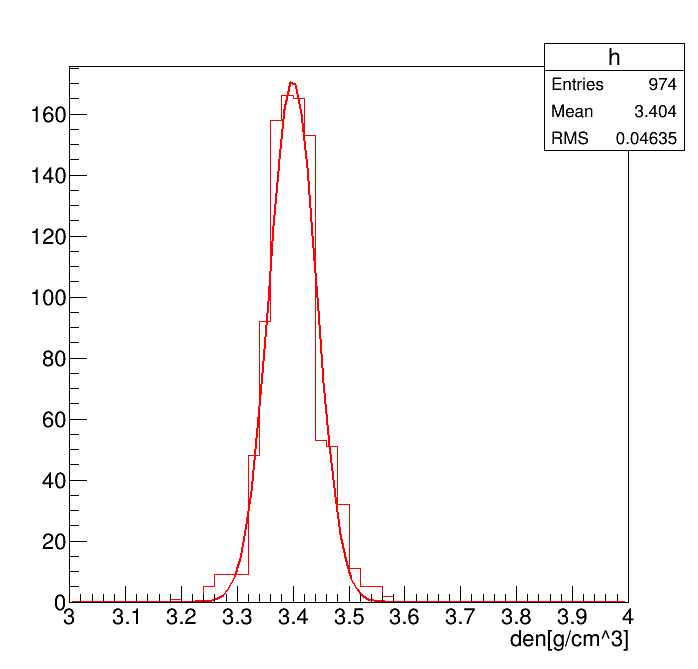
\includegraphics[width=70mm]{thick75_den.png}
  \caption{ヒストグラム\label{fig:hisuto}}
\end{figure}
\begin{table}[htbp]
  \centering
  \caption{J-PARC E07実験で使用した原子核乾板の密度\label{tab:compare_E07_12}}
  \begin{tabular}{c|c|c}
     &1stRun [g/cm$^3$]&2ndRun [g/cm$^3$]\\
  \hline
  \hline
  可塑剤6.0cc 厚型乾板 & 3.48 $\pm$ 0.04 & 3.43 $\pm$ 0.05 \\
  可塑剤7.5cc 厚型乾板 & 3.41 $\pm$ 0.07 & 3.40 $\pm$ 0.04 \\
 薄型乾板 & 3.73 $\pm$ 0.16 & 3.74 $\pm$ 0.13 \\
  \hline
  \end{tabular}
\end{table}
\begin{figure}[htbp]
  \centering
     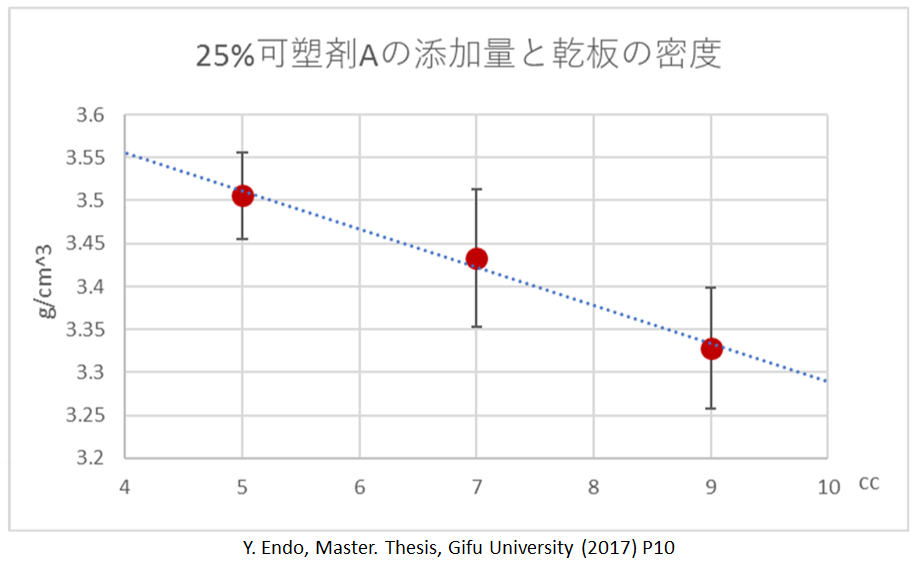
\includegraphics[width=140mm]{kasozai.png}
  \caption{可塑剤Aの添加量に対する原子核乾板の密度\label{fig:kasozai}}
\end{figure}
\newpage
\subsection{現像}
\begin{itemize}
 \item 原子核乾板すべて現像している。
 \item 現像の行程
 \item 1stRunは●年に●枚終了、2ndRunは●年に●枚終了予定
 \item 現像の詳細な記述は大橋修論に記載する。 それなら実施環境とどれくらい行ったのかを記載すればいいかな。
\end{itemize}
\subsubsection{原理}
原子核乾板の現像には予浸(presoark)、現像(Cold.dev Hot.dev)、現像(Cold.dev Hot.dev)、停止(Stop)、定着(Fix2/4、Fix4/4)、水洗(Wash)の工程がある。
原子核乾板はこの順で工程を実施することで、記録した荷電粒子飛跡を顕微鏡で観察できるようになる。
\par
予浸(presoark)とは、原子核乾板に水分を吸収させる工程である。
beam照射の際も原子核乾板は乾燥した状態で実施している。
乾燥した状態では、これ以降の工程で使用する現像液や薬品が浸透しにくくなり、現像のムラが発生する恐れがある。
そのため、現像液が原子核乾板の表面だけでなく内部にも浸透しやすくするために、乾燥した原子核乾板に水分を吸収させる。
\par
現像(Cold.dev Hot.dev)とは、原子核乾板中で荷電粒子により生成された銀粒子の形成を促進する工程である。
\par
停止(Stop)とは、現像の工程で促進された銀粒子の形成促進の反応を停止させる工程である。
現像では荷電粒子によって形成された銀粒子のみ選択的に形成促進させている。
しかし、原子核乾板中には大量の銀粒子が存在しているため、銀粒子の形成促進を行いすぎるとすべての銀粒子が現像されてしまう。
我々は荷電粒子によって形成された銀粒子のみを観察する必要があるため、停止の工程で現像を止め、必要な情報のみ残された状態にする。
\par
定着(Fix2/4、Fix4/4)
\par
水洗(Wash)
\subsubsection{実施環境}
E07実験でbeam照射された全●●枚の原子核乾板は岐阜大学内に建てられたDH核実験棟にて現像をした。
図●は現像を実施した環境を示している。
大きな浴槽一つ一つに液を貯め、図●のようにした原子核乾板を一定時間各工程の浴槽に漬けることで現像する。
表●は各工程にて何をどれくらい溶解させているのかを示したものである。
また、図●は現像のタイムテーブルである。
この図の通りに原子核乾板を液に漬け、現像した。
\begin{figure}[htbp]
  \centering
      \begin{tabular}{c}
        % 1枚目の画像
        \begin{minipage}{0.5\hsize}
          \centering
            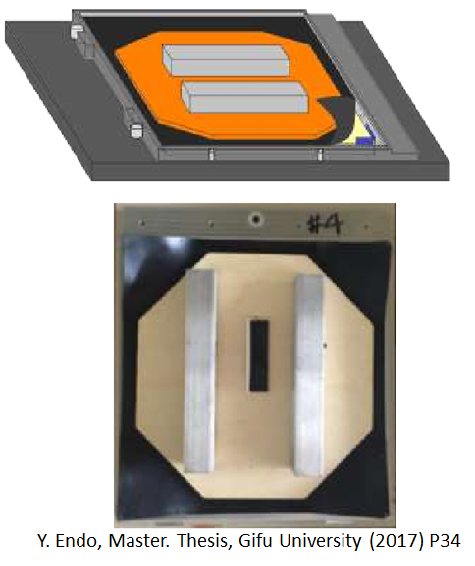
\includegraphics[clip, width=70mm]{tezyun_8.png}
            \hspace{1.6cm} 
            \caption{現像環境\label{fig:gennzou_bath}}
        \end{minipage}
        
        % 2枚目の画像
        \begin{minipage}{0.5\hsize}
          \centering
            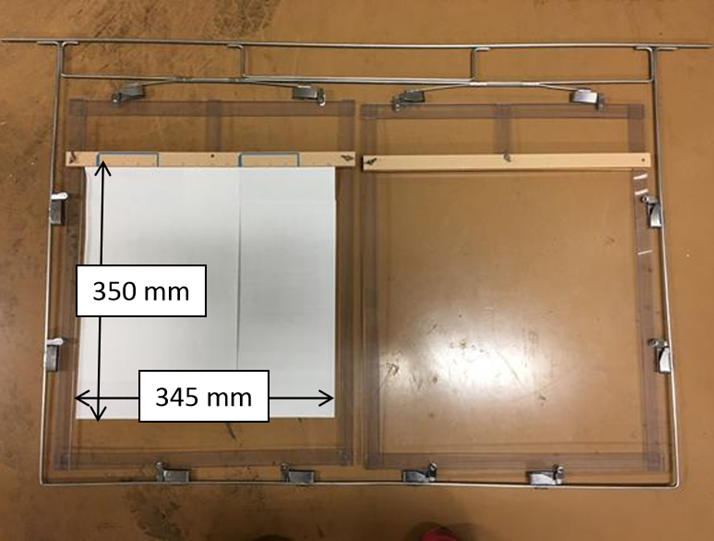
\includegraphics[clip, width=70mm]{refresh_hanga.png}
            \hspace{1.6cm} 
            \caption{乾板ハンガー\label{fig:emulsion_hanga}}
        \end{minipage}
    
      \end{tabular}
\end{figure}
\begin{table}[htbp]
  \centering
  \caption{E07実験における現像タイムテーブル\label{tab:gennzou_timetable}}
  \begin{tabular}{c|c|c|c|c}
     &Thick plates&Thin plates&液温&薬品\\
  \hline
  \hline
 Presoak & 2 h & 10 min & $5\ {}^\circ\mathrm{C}$ & Na$_2$SO$_4$\\
  可塑剤7.5cc 厚型乾板 & 3.41 $\pm$ 0.07 & 3.40 $\pm$ 0.04 \\
 薄型乾板 & 3.73 $\pm$ 0.16 & 3.74 $\pm$ 0.13 \\
  \hline
  \end{tabular}
\end{table}


\newpage
\section{荷電粒子飛跡追跡の自動化}
\subsection{目的}
E373実験では人が約2.0×10$^4$本の$\Xi$$^-$候補を顕微鏡を使い静止点まで追跡した。
この追跡には約数年が必要となった。
先に記述したが、今年度実施されたJ-PARC E07実験ではハイブリッド-エマルジョン法によりE373実験の約10倍の統計量を検出することを目標にしている。
今回実施されたE07実験では、E373実験より精度の高い検出機であるSSDを使うことで追跡するべき候補飛跡を増やさないようにしている。
カウンターの情報と原子核乾板に記録された飛跡を一対一対応を付ける。
しかし、その条件であっても追跡すべき$\Xi$$^-$候補飛跡がE373実験の本数を超えることが予想されるため、
機械が自動で飛跡を静止点まで追跡するプログラムが必要になった。
\par
この章では$\Xi$$^-$候補飛跡のために使用・開発した要素技術について記述する。
SSDとE373実験の際に使用された検出機の精度をまとめた表を示す。
\subsection{$\Xi$$^-$候補&beam認識に用いる画像処理}
\subsubsection{コントラスト処理}
原子核乾板中を撮影した画像は、画像を撮影した原子核乾板の位置により見え方が異なる。
図\ref{fig:diff_contrust}は同一乾板内で撮影した写真で、視野中心に見えるのは追跡対象にしている$\Xi$$^-$候補飛跡である。
二つの写真の違いは原子核乾板の位置で、左が上側乳剤層、右が下側乳剤層で撮影したものである。
図より撮影地点が異なれば画像のコントラストが大きく異なることが分かる。
そこで原子核乾板中で撮影した画像を、撮影地点によらず飛跡情報を取得するために画像のコントラストの違いをなくす必要がある。
\par
コントラストとは、画像の濃淡情報の分布の広さに関する性質で、画像の最大輝度を$I_{max}$、最小輝度を$I_{min}$とするとき式(\ref{eq:cont})で表す。
コントラスト処理に使う変化式はまた調べて記入する。
\begin{equation}
  C = \frac{I_{max} - I_{min}}{I_{max} + I_{min}}
\label{eq:cont}
\end{equation}
\begin{figure}[htbp]
  \centering
      \begin{tabular}{c}
        % 1枚目の画像
        \begin{minipage}{0.5\hsize}
          \centering
            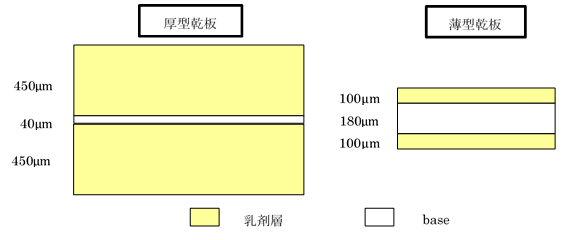
\includegraphics[clip, width=60mm]{emulsionorder.png}
            \hspace{1.6cm} (a)上側乳剤層中の$\Xi$$^-$候補飛跡
        \end{minipage}

        % 2枚目の画像
        \begin{minipage}{0.5\hsize}
          \centering
            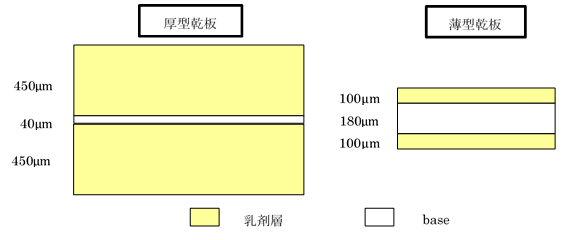
\includegraphics[clip, width=60mm]{emulsionorder.png}
            \hspace{1.6cm} (b)下側乳剤層中の$\Xi$$^-$候補飛跡
        \end{minipage}
    
      \end{tabular}
      \caption{撮影地点によるコントラストの違い\label{fig:diff_contrust}}
\end{figure}
\par
画像のコントラストをよくするために用いる式は以下の通りである。
図\ref{fig:do_contrust_beforeandafter}はこの式を使用して画像にコントラスト処理を施した画像である。
図のc、dを比較すると、コントラスト処理により画像の輝度値の明暗の幅が広がったことが分かる。
\begin{figure}[htbp]
  \centering
      \begin{tabular}{c}
        % 1枚目の画像
        \begin{minipage}{0.5\hsize}
          \centering
            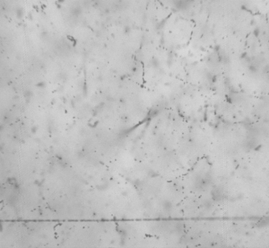
\includegraphics[clip, width=60mm]{row.png}
            \hspace{1.6cm} (a)コントラスト処理前
        \end{minipage}
        
        % 2枚目の画像
        \begin{minipage}{0.5\hsize}
          \centering
            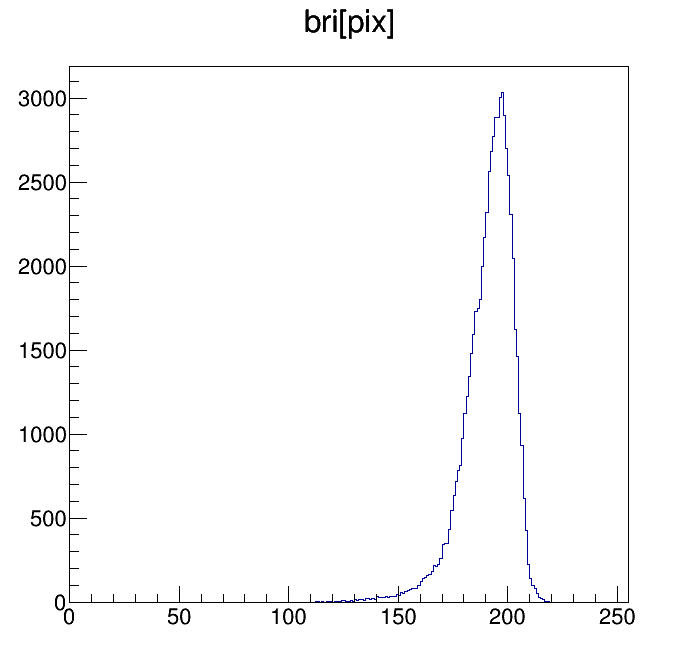
\includegraphics[clip, width=60mm]{row_hist.png}
            \hspace{1.6cm} (b)(a)の輝度値分布
        \end{minipage}
        \\
        \\
        % 3枚目の画像
        \begin{minipage}{0.5\hsize}
          \centering
              \includegraphics[clip, width=60mm]{cont.png}
              \hspace{1.6cm} (c)コントラスト処理後
          \end{minipage}
          
        % 4枚目の画像
        \begin{minipage}{0.5\hsize}
          \centering
              \includegraphics[clip, width=60mm]{cont_hist.png}
              \hspace{1.6cm} (d)(c)の輝度値分布
        \end{minipage}
    
      \end{tabular}
      \caption{コントラスト処理によるコントラストの違い\label{fig:do_contrust_beforeandafter}}
\end{figure}
\subsubsection{ガウシアンフィルタ処理}
撮影された画像には意図していないノイズが含まれている。
機械に飛跡を認識させるために、画像を構成する1つ1つのpixelに割り当てられた輝度値情報を利用する。
画像処理によりなめらかな濃淡変化画像に与え、画像に含まれるノイズなどの不要な濃淡変動を軽減する。(平滑化)
\par
ガウシアンフィルタとは、画像の平滑化を行うために設定する平滑化フィルタの一例である。
フィルタによって覆われる領域内の画素の値がフィルタの原点に近いほど大きな重みをつけるが、この重みをガウス分布に近づけたフィルタを指す。
その際の二次元ガウス分布は式(\ref{eq:gausu})で表される。
\begin{equation}
  h_g(x,y) = \frac{1}{2\pi\sigma^2}exp(-\frac{x^2 + y^2}{2\sigma^2})
\label{eq:gausu}
\end{equation}
画像中のある画素を中心に指定範囲(カーネルサイズ)内で注目画素に近いほど輝度値の平均値を計算するときの重みを大きくするように処理をかけることである。
式は次の通りである。
この式を使い、処理を実施した。
\begin{figure}[htbp]
  \centering
      \begin{tabular}{c}
        % 1枚目の画像
        \begin{minipage}{0.5\hsize}
          \centering
            \includegraphics[clip, width=60mm]{cont.png}
            \hspace{1.6cm} (a)ガウシアンフィルタ処理前
        \end{minipage}
        
        % 2枚目の画像
        \begin{minipage}{0.5\hsize}
          \centering
            \includegraphics[clip, width=60mm]{cont_hist2.png}
            \hspace{1.6cm} (b)(a)の中央行の輝度値
        \end{minipage}
        \\
        \\
        % 3枚目の画像
        \begin{minipage}{0.5\hsize}
          \centering
              \includegraphics[clip, width=60mm]{gau2.png}
              \hspace{1.6cm} (c)ガウシアンフィルタ処理後
          \end{minipage}
          
        % 4枚目の画像
        \begin{minipage}{0.5\hsize}
          \centering
              \includegraphics[clip, width=60mm]{gau2_hist.png}
              \hspace{1.6cm} (d)(c)の中央行の輝度値
        \end{minipage}
    
      \end{tabular}
      \caption{ガウシアンフィルタ処理による輝度値の違い\label{fig:do_gau_beforeandafter}}
\end{figure}
\subsubsection{画像の白黒反転}
次の二値化処理を実施するため、画像の白黒を反転させる必要がある。
ガウシアンフィルタ処理を施した画像から、コントラスト処理を施した画像の輝度値の差を取ることで白黒を反転する。
図\ref{fig:do_gau_beforeandafter}(c)の画像の輝度値から(a)の輝度値情報を引いて作成したのが図\ref{fig:do_sub}である。
図\ref{fig:do_sub}を見れば分かるように差分を取ることで、黒色であった部分が白色に反転した。
\begin{figure}[htbp]
  \centering
      \begin{tabular}{c}
        % 1枚目の画像
        \begin{minipage}{0.5\hsize}
          \centering
            \includegraphics[clip, width=60mm]{sub.png}
            \hspace{1.6cm} (a)図\ref{fig:do_gau_beforeandafter}(c)-(a)
        \end{minipage}

        % 2枚目の画像
        \begin{minipage}{0.5\hsize}
          \centering
            \includegraphics[clip, width=60mm]{sub_hist.png}
            \hspace{1.6cm} (b)(a)の中央行の輝度値
        \end{minipage}
    
      \end{tabular}
      \caption{輝度値差分処理後の画像\label{fig:do_sub}}
\end{figure}
\subsubsection{二値化}
図\ref{fig:do_sub}を見ると、視野中心にある飛跡情報以外に多くの輝度値情報が記録されていることが分かる。
これらの情報は飛跡追跡を実施するのに不必要であり、飛跡の誤検出を招く恐れがある。
そこで、二値化処理により指定した輝度値以下のピクセルの輝度値をゼロにする。
これにより飛跡以外の不要な輝度値情報を消す。
\par
図\ref{fig:do_thre}は二値化処理前後の画像とその指定した行の輝度値を示したものである。
閾値を70に設定して二値化処理を実施した。
図より二値化処理により飛跡以外の不要な輝度値情報が減少したことが分かる。
\begin{figure}[htbp]
  \centering
      \begin{tabular}{c}
        % 1枚目の画像
        \begin{minipage}{0.5\hsize}
          \centering
            \includegraphics[clip, width=60mm]{thre.png}
            \hspace{1.6cm} (a)図\ref{fig:do_sub}(a)の二値化処理後画像
        \end{minipage}

        % 2枚目の画像
        \begin{minipage}{0.5\hsize}
          \centering
            \includegraphics[clip, width=60mm]{thre_hist.png}
            \hspace{1.6cm} (b)(a)の中央行の輝度値
        \end{minipage}
    
      \end{tabular}
      \caption{二値化処理後の画像\label{fig:do_thre}}
\end{figure}
\subsection{座標変換}
\begin{itemize}
    \item affine変換について書く。
    \item 追跡の際に考える必要のある座標系について書く。
    \item それらの座標系をつなぐためにaffine変換をつかい、目的の飛跡の位置に行くことが必要である。
\end{itemize}
追跡するべき飛跡情報はDetector座標系(SSD座標系)、Grid座標系(現像前座標系)、Stage座標系(現像後座標系)の3座標系で表すことができる。
Detector座標系はSSDの検出座標系である。
Grid座標系はemulsionにbeam照射をして現像をする前の座標系である。
Stage座標系は顕微鏡で原子核乾板を観察する際の座標系である。
\par
SSDで検出された候補飛跡はDetector座標系で記録されている。
検出された候補飛跡を原子核乾板で観察するためにはDetector座標系、Grid座標系、Stage座標への変換を適切に行う必要がある。
その座標間の変換を適切に行うためにaffine変換を使用する。
\par
\begin{equation}
  \left(
    \begin{array}{c}
    x \\
    y
    \end{array}
  \right)
  =
  \left(
    \begin{array}{cc}
      a & b \\
      c & d
    \end{array}
  \right)
  \left(
    \begin{array}{c}
      X \\
      Y
    \end{array}
  \right)
  +
  \left(
    \begin{array}{c}
      p \\
      q
    \end{array}
  \right)
\label{eq:affine}
\end{equation}
式(\ref{eq:affine})を使い、座標変換を行う。
x,yが座標変換後の座標、X,Yが座標変換前の座標、2行2列の行列が線形変換について、p,qが平行移動の成分になる。
x,yとX,Yが対応している地点を3点以上検出し、式を解くことで各変換パラメータを出取得できる。
その変換パラメータを使い、対応がついていない地点の座標を推定する。
\subsection{自動追跡の要素技術}
\subsubsection{beamパターンマッチ}
カウンターと原子核乾板の位置ズレや乾板間の位置ズレを正確に取得する手法としてbeamパターンマッチという手法が開発された。[大輔修論]
図●はパターンマッチの模式図である。
系1と系2に記録されたbeamの形状が変化しておらず、互いの系において座標が異なる場合、使用できる。
パターンマッチをするために系1と系2に記録されたbeamの座標の差分を総当たりで計算をする。
系1のbeam一点に対して複数のbeamの位置差をとることになるので、計算後系1のbeam一点に対して複数のベクトルが引けることになる。
この作業をすべてのbeamで実施したのち、そのすべてのベクトルを集計する。
このとき、系1と系2がある数値分ずれている場合、その数値分ずれたベクトルが多く集計され、その他のベクトルはほとんど集計されないことになる。
そのベクトルの集計でヒストグラム作成した場合このようにpeakが出現する。
これにより、系1と系2の間に一定値のずれが存在している場合の位置ズレが取得できる。
\subsubsection{P-barパターンマッチ}
\begin{itemize}
    \item SSDとemulsionの位置ズレを取得するのに必要。
    \item 乾板の四隅に照射されているものを使う。(なぜP-barを使うのか、どのようにP-barが照射されているか確認する。)
    \item どのようにP-barを取得するのか(スキャンする場所等を書く)を書く。
    \item 四隅のうち3点箇所でパターンマッチがとれればズレが取得できる。(精度について書く。)
\end{itemize}
原子核乾板にはSSDとemulsionの照射時の位置差を取得するために反陽子ビームが照射されている。
照射されているのは乾板の四つ角1cm1cmの領域であり、SSDと原子核乾板に対して垂直に照射されている。
照射されている反陽子beamの濃度は1平方センチあたり10$^4$である。
K$^-$beamは乾板に対して10$^6$照射されており、SSDとemulsionのパターンマッチをするには密に照射されているためp-barが必要になる。
(おそらくSSDのワイヤーの張る間隔が10の6乗より疎であるから、K-では不可能)
\par
角から1cmずつ内陸側に移動し、そこで5mm×5mmの領域をスキャンする。
上側乳剤層と下側乳剤層をスキャンし、baseを挟んで接続された垂直なbeamを選び出すことで、原子核乾板薄型一枚目での飛跡集団のパターンを取得する。
また、SSDに記録された垂直な飛跡集団を選び出すことでSSDに記録された飛跡集団のパターンを取得する。
\par
SSDと原子核乾板薄型一枚目での飛跡集団同士でパターンマッチを行うことで、SSDとemulsionの座標系の対応をつける。
\subsubsection{$\Xi$$^-$候補飛跡の選択}
\begin{itemize}
    \item 追跡の際に考える必要のある座標系について書く。
    \item それらの座標系をつなぐためにaffine変換をつかい、目的の飛跡の位置に行くことが必要である。
\end{itemize}
追跡するために、SSDで検出した$\Xi$$^-$候補とpl01に記録された荷電粒子飛跡の対応をつける。
先述したP-barパターンマッチにより、SSDと原子核乾板の座標の対応がついている。
SSDで検出された$\Xi$$^-$候補の位置情報と角度情報を使い、$\Xi$$^-$候補の位置を薄型原子核乾板1枚目のbase上面まで外挿する。
これにより$\Xi$$^-$候補の薄型原子核乾板1枚目のbase上面における位置がおおよそ分かる。
この薄型原子核乾板1枚目のbase上面における位置情報と角度情報を合わせてprediction(pred)とする。
\par
predの座標を中心にして$\Xi$$^-$候補の角度により、原子核乾板中をスキャンする範囲を設定する。
設定した範囲を元に、原子核乾板の上側乳剤層、下側乳剤層をscanし、原子核乾板中に記録されている荷電粒子飛跡を検出する。
検出した飛跡の中から、baseをまたいで繋がるものを薄型一枚目を通過している飛跡(basetrack)として記録する。
basetrackは位置情報、角度情報を持っている。
predとbasetrackの中から、角度がおおよそ似ている飛跡を追跡対象として下流の原子核乾板に接続し、飛跡追跡を行う。
\subsubsection{K$^-$beamパターンマッチ}
\begin{itemize}
    \item emulsionとemulsionの位置ズレを補正するために行う。
    \item これにより、例pl01で記録された飛跡とpl02で記録された飛跡の対応付けをする。
    \item どこをスキャンして、どのようになるのかを書く。模式図を書く。
\end{itemize}
beam照射は、エマルジョンカセットに13枚の原子核乾板を入れ、真空度を保ちbeam照射中に原子核乾板がずれないようにして実施した。
しかし、原子核乾板一枚一枚違いがあり、現像の前後での変形も一様ではないため、
上流の原子核乾板の位置情報と下流の原子核乾板の位置情報は、原点を照射したGridマークの中心にしたときに対応しない。
そこで、beam照射時に原子核乾板に対して垂直に照射されているK$^-$beamを使い、上流乾板と下流乾板の位置の対応をつける。
\subsubsection{表面認識}
\begin{itemize}
    \item 乳剤層と非乳剤層の境界面を取得するために行う。
    \item 乾板中の位置における輝度値の違いを示す。
\end{itemize}
原子核乾板中の飛跡を認識するために、原子核乾板の乳剤と非乳剤の地点を正確に捉える必要がある。
図\ref{fig:do_hyoumenn_outin_image}(a)、(b)は原子核乾板の乳剤層と非乳剤層で撮影した画像である。
乳剤中で撮影した画像の場合は飛跡等が記録されているが、非乳剤層では記録されない。
この画像に対して画像処理を実施したのが図\ref{fig:do_hyoumenn_outin_image}(c)、(d)である。
図より乳剤層か非乳剤層かにより画像処理後の画像中で輝度値情報を持つピクセルの数が異なることが分かる。
輝度値情報を持つピクセルの数により乳剤層か否かを判断する。
これが表面認識である。
\begin{figure}[htbp]
  \centering
      \begin{tabular}{c}
        % 1枚目の画像
        \begin{minipage}{0.5\hsize}
          \centering
            \includegraphics[clip, width=60mm]{cont.png}
            \hspace{1.6cm} (a)乳剤層
        \end{minipage}
        
        % 2枚目の画像
        \begin{minipage}{0.5\hsize}
          \centering
            \includegraphics[clip, width=60mm]{cont_hist2.png}
            \hspace{1.6cm} (b)非乳剤層
        \end{minipage}
        \\
        \\
        % 3枚目の画像
        \begin{minipage}{0.5\hsize}
          \centering
              \includegraphics[clip, width=60mm]{gau2.png}
              \hspace{1.6cm} (c)画像処理後(乳剤層)
          \end{minipage}
          
        % 4枚目の画像
        \begin{minipage}{0.5\hsize}
          \centering
              \includegraphics[clip, width=60mm]{gau2_hist.png}
              \hspace{1.6cm} (d)画像処理後(非乳剤層)
        \end{minipage}
    
      \end{tabular}
      \caption{原子核乾板内外での違い\label{fig:do_hyoumenn_outin_image}}
\end{figure}
\par
顕微鏡操作し、乾板中の焦点が合っている箇所のZ軸だけを動かし3 µm間隔で画像を撮影し、画像処理を実施する。
その操作を行い、輝度値情報を持つピクセルの数を縦軸、Z座標を横軸に取り作成したのが図\ref{fig:hyoumenn_kidoti}である。
図より輝度値が急激に変化している箇所が4箇所ほど存在している。
その部分が乳剤層と非乳剤層の境界になる。
各境界面を認識する閾値を設定し、乳剤層である座標を求める。
\begin{figure}[htbp]
  \centering
     \includegraphics[width=140mm]{kasozai.png}
  \caption{原子核乾板の撮影か所による輝度値情報の推移\label{fig:hyoumenn_kidoti}}
\end{figure}
\subsubsection{荷電粒子飛跡追跡}
荷電粒子飛跡追跡の飛跡を検出する部分と追跡する際の顕微鏡の駆動について記述をする。
\par
原子核乾板中に記録された荷電粒子飛跡を認識するために最も重要なのは、荷電粒子飛跡の重心を正確にとらえることである。
飛跡の重心をとらえるために、乾板中の荷電粒子飛跡の写真を撮影し、上述した画像処理を用いて画像から重心を取得する。
\par
追跡する荷電粒子の位置情報から、飛跡が画像の視野中心にあるとする。
追跡する荷電粒子の角度情報をもとに飛跡に沿い、常に視野中心にあるように顕微鏡のx,y方向を駆動させながら、z=-4 µm間隔で10枚の画像を撮影する。
10枚の画像すべてに画像処理(●参照)を施し、輝度値情報が反転した画像に変換する。
追跡の際に、荷電粒子飛跡が常に画像中心にあるようにして撮影をしているので、画像中に記録された輝度情報をすべて使うのは誤検出につながる。
そのため画像処理の際に、画像処理をする領域(mask)を設定し、領域外の輝度情報を消した画像にしている。
\par
追跡には、上述した表面認識、K$^-$beamパターンマッチによる$\Xi$$^-$候補飛跡の乾板間接続が成功し、
追跡する荷電粒子飛跡の位置、角度情報が必要である。
表面認識により、原子核乾板の各境界面
\par
追跡には角度と位置情報が必要であり、追跡のはじめに画像の視野中心に荷電粒子飛跡があることが求められる。





\newpage
\section{E07乾板における開発プログラムでの追跡実績}

\newpage
\section{まとめ}

\section*{付録}
\addcontentsline{toc}{section}{付録}
これは付録でいいかな???
原子核乾板中に記録されたHyper核eventを解析するためには記録されている原子核乾板の密度が重要になる。
記録された飛跡の飛程からエネルギーを算出する際に乾板の密度が必要になるからである。
現在核種が一意に決定されている'NagaraEvent'の解析にはevent付近に記録されたα崩壊飛跡を50例使用し、乾板の密度を計算して○.○○とした。
\par
表○はNagaraの各trackの長さ、角度を示している。
trackの長さ、角度が一定で、原子核乾板の密度を変化させたときBΞがどれだけ変化するかを確認した。
図●はその変化を示している。
図から分かるように密度の変化によってBΞは大きく変化する。
そのため原子核乾板の密度を正確に求めること、密度が解析において非常に重要であることが分かる。
\par
図を入れる。
\par
\begin{figure}[htbp]
  \centering
      \begin{tabular}{c}
        % 1枚目の画像
        \begin{minipage}{0.5\hsize}
          \centering
            \includegraphics[clip, width=60mm]{1stRun_thin_den.png}
            \hspace{1.6cm} (a)1stRun 厚形乾板密度 可塑剤6.0cc
        \end{minipage}
        
        % 2枚目の画像
        \begin{minipage}{0.5\hsize}
          \centering
            \includegraphics[clip, width=60mm]{2ndRun_thin_den.png}
            \hspace{1.6cm} (b)2ndRun 厚形乾板密度 可塑剤6.0cc
        \end{minipage}\\

	 \\
        % 3枚目の画像
        \begin{minipage}{0.5\hsize}
          \centering
              \includegraphics[clip, width=60mm]{1stRun_thin_den.png}
              \hspace{1.6cm} (c)1stRun 厚形乾板密度 可塑剤7.5cc
          \end{minipage}
          
        % 4枚目の画像
        \begin{minipage}{0.5\hsize}
          \centering
              \includegraphics[clip, width=60mm]{2ndRun_thin_den.png}
              \hspace{1.6cm} (d)2ndRun 厚形乾板密度 可塑剤7.5cc
        \end{minipage}
    
      \end{tabular}
      \caption{厚形乾板の密度比較\label{fig:compare_thick_den}}
\end{figure}
\begin{figure}[htbp]
  \centering
      \begin{tabular}{c}
        % 1枚目の画像
        \begin{minipage}{0.5\hsize}
          \centering
            \includegraphics[clip, width=60mm]{1stRun_thin_den.png}
            \hspace{1.6cm} (a)1stRun 薄型密度
        \end{minipage}
        
        % 2枚目の画像
        \begin{minipage}{0.5\hsize}
          \centering
            \includegraphics[clip, width=60mm]{2ndRun_thin_den.png}
            \hspace{1.6cm} (b)2ndRun 薄型密度
        \end{minipage}
    
      \end{tabular}
      \caption{薄型乾板の密度比較\label{fig:compare_thin_den}}
\end{figure}
\newpage
\section*{謝辞}
\addcontentsline{toc}{section}{謝辞}
ああああああああああああああああああああああああああ
\begin{thebibliography}{99}
\bibitem{Nagara} 「Double-$\Lambda$Hypernuclei observed in a hybrid emulsion experiment」PHYSICAL REVIEW C NUCLEAR PHYSICS Vol.88,No.1, July 2013
\bibitem{Nagara2} 「”NAGARA event”が語る相互作用―KEK-PS E373 ダブルハイパー核実験―」仲澤和馬(岐阜大学)、高橋仁(京都大学)、PS-E373 共同実験グループ 高エネルギーニュース Vol.20 No.5 p.206 2002
\bibitem{takusann} 学位論文「大規模実験用高性能原子核乾板OPERA Filmの開発」第四章 Refresh処理 名古屋大学大学院理学研究科素粒子宇宙物理学専攻F研究室 中村琢 著(2005年)
\end{thebibliography}
\end{document} 